\documentclass[12pt]{article}
\usepackage[natbib=true,style=authoryear]{biblatex}
  \addbibresource{references.bib}
  \setlength\bibitemsep{0pt}
\usepackage{pgf}
\usepackage[colorlinks,citecolor=blue,linkcolor=black,bookmarks=false,hypertexnames=true]{hyperref}
\usepackage{url}
\usepackage[inline]{enumitem}
\usepackage{float}
\usepackage[bottom,perpage,multiple]{footmisc}
\usepackage{booktabs}
\usepackage{graphicx}
\usepackage{xcolor}
\usepackage{setspace}
  \setstretch{1.1}
\usepackage{enumitem}
\usepackage{caption}
\usepackage{xcolor}
\usepackage[top=1.3in, left=1.4in, includefoot]{geometry}
\setlist{nosep}
\usepackage{xcolor}
\usepackage{algorithm}
\usepackage{algpseudocode}
\usepackage{multicol}
\usepackage[T1]{fontenc}
\usepackage[utf8]{inputenc}
\usepackage{charter}
\usepackage{listings}
\usepackage{authblk}

\definecolor{codegreen}{rgb}{0,0.6,0}
\definecolor{codegray}{rgb}{0.5,0.5,0.5}
\definecolor{codepurple}{rgb}{0.58,0,0.82}
\definecolor{backcolour}{rgb}{0.95,0.95,0.92}

\lstdefinestyle{mystyle}{
	backgroundcolor=\color{backcolour},
	commentstyle=\color{codegreen},
	keywordstyle=\color{magenta},
	numberstyle=\tiny\color{codegray},
	stringstyle=\color{codepurple},
	basicstyle=\sffamily\footnotesize,
	breakatwhitespace=false,
	breaklines=true,
	captionpos=b,
	keepspaces=true,
	numbers=left,
	numbersep=5pt,
	showspaces=false,
	showstringspaces=false,
	showtabs=false,
	tabsize=2
}

\lstset{style=mystyle}

\newcommand{\pattern}[3]{
	{\bf #2. #1} \\
	{\it Description:} #3 \\
}

\newcommand{\todo}{\textcolor{red}{\textbf{TODO}}}
\tolerance=800

\usepackage{pgfplots}
%\DeclareUnicodeCharacter{2212}{-}
\usepgfplotslibrary{groupplots,dateplot}
\usetikzlibrary{patterns,shapes.arrows}
\pgfplotsset{compat=newest}

\usepackage{url}
\renewcommand*{\bibfont}{\footnotesize}

\title{
  
\includegraphics[height=100pt]{logo.png}\\
  \vspace{10pt}
  \textsc{Aibolit:}\\
  Static Analysis
  Using Machine Learning}
\author{Yegor Bugayenko, Anton Cheshkov, Ekaterina Garmash, Andrey Gusev, Yaroslav Kishchenko, Pavel Lukyanov, Evgeny Maslov, Vitaly Protasov}
\affil{Huawei Technologies Co., Ltd. \\ System Programming Lab \\ Russian Research Institute (RRI) \\ Moscow, Russia}

\begin{document}

\maketitle

\pagebreak

\begin{abstract}

Aibolit is a next generation static analyzer powered by machine learning.
Aibolit gives recommendations to developers to avoid specific software patterns
in order to improve quality of the source code. Aibolit can be extended by adding
custom patterns and quality metrics of choice. In this paper, we explain
how Aibolit works and how it differs from other static analyzers.

\end{abstract}

\pagebreak

\section{Introduction}
\label{sec:intro}
% SPDX-FileCopyrightText: Copyright (c) 2019-2025 CQFN.org
% SPDX-License-Identifier: MIT

Insufficient software quality may result in increased development costs and
negatively affect customer satisfaction ~\citep{The_Economics_of_Software_Quality}.
\textit{Static code analysis} develops techniques to help detect software quality
issues prior to program execution. It has its practical application in various developer's tools. There are both open source\footnote{PMD: \url{http://pmd.sourceforge.net/}, Rubocop: \url{https://github.com/rubocop-hq/rubocop},
PHPCS: \url{https://github.com/squizlabs/PHP_CodeSniffer}
FindSecBugs: \url{https://find-sec-bugs.github.io/}, ESLint: \url{https://eslint.org/}, Checkstyle: \url{https://checkstyle.sourceforge.io/}.}
(PMD, Rubocop, PHPCS, FindSecBugs, ESLint, Checkstyle, to name a few) and commercial\footnote{IBM Security AppScan: \url{https://www.hcltechsw.com/wps/portal/products/appscan},
PVS-Studio: \url{https://www.viva64.com/en/pvs-studio/},
SonarQube: \url{https://www.sonarqube.org/},
Parasoft: \url{https://www.parasoft.com/}}
(IBM Security AppScan, PVS-Studio, SonarQube, Parasoft) static analyzers
on the market.

Static code analysis can be applied to improve an \textit{internal} and an
\textit{external} quality of software \citep{Ilyas2016StaticCA}. External
quality is related to defects encountered by the end user of the software
product. Within internal quality, two important subcategories are
\textit{functional quality} and \textit{maintainability}. Functional quality is
about code correctness and compliance with the functional software
specifications \citep{Farhan}. Code maintainability is about how easy it is to
analyze, modify and adapt given software \citep{Mohammadi2013AnAO}.

Functional quality aspects are typically quite susceptible to formal definition
and quantification.
% (\todo: examples!!).
Functional quality is also an essential
requirement in any domain of software development. On the other hand,
maintainability is a lot less straightforward to formally specify or quantify.
%\todo: refs.
Also, in certain applications it appears less important than
functional correctness, although in business domain it is recognized as an
essential property.
% (\todo: ref).
As a result, there are currently a lot more
research and practical tools addressing functional quality aspects of code than
maintainability \citep{Overview_Static_Code_Analysis_in_Software_Development}.
Another aspect of static analysis tools that may have hindered their application
to maintainability, is that they are predominantly rule-based. Since there has
not yet been a consensus on how to formalize maintainability, it is challenging
to devise a set of formal rules to detect it.

We designed our new tool Aibolit to help developers identify patterns in their
code  that may cause maintainability issues. It is a next generation static
analysis tool that uses a machine learning (ML) model as an underlying quality
prediction mechanism. From the perspective of ML, our product is a recommender
system. For a given class file, it gives suggestions to the developer to alter
their code. The recommendations come in the form of \textit{code patterns} that
are detected in the code and advised to be removed.

Our choice to design Aibolit as a ML-based system alleviates some important
shortcomings of rule-based static analyzers. By design, ML algorithms capture
statistical relations in the external world (data). Therefore, they can be a
good way to model imprecisely and subjectively defined properties of code, such
as its maintainability. Moreover, rule-based system are known to not scale well
to the diversity of empirically observed cases, and they tend to get very hard
to extend and maintain \citep{LenatFeigenbaum1987}. The ML
approach does not require
manual system adaptation as new observations or new features (patterns) come
along. In fact, Aibolit provides an easy way for developers to integrate a code
pattern of their liking into the recommender system and to analyze the pattern`s
impact on code quality.






% This document explains how Aibolit works  and what makes it novel and
% different from other static analyzers (Section~\ref{sec:method}).
% We further show how Aibolit can be extended
% with custom patterns and metrics. We discuss the current shortcomings and the way
% they can be addressed in future work (Section~\ref{sec:conclusion}).



\section{Software quality and patterns}
\label{sec:related}
There are many definitions of a defect.  
\citet{5989519} says that defect is ``a fault, bug, inaccuracy or lack of expected 
functionality in a project artifact.'' 
\citet{Assurance} says that it is ``a problem 
(synonym of fault) which, if not corrected, 
could cause an application to either fail or to produce incorrect results.''

Defects and software quality are directly related. There are multiple studies 
of defect types, their impact, complexity, 
root causse and other characteristics,~\citet[e.g.][]{10.1145/69605.2085, 
10.5555/256664.256773, 10.1145/390016.808455, Glass1981PersistentSE, 
10.1145/1353535.1346323, 10.1007/s10664-013-9258-8, catolino2019bugs}.
There are a few common preventive ways to deal with defects, like 
static code analyzers, testing software, or peer code review. 

Static code analyzer 
is a tool that helps find defects before a program is executed. 
Such an analyzer inspects various program representations, for example 
Abstract Syntax Tree (AST), Control Flow Graphs (CFG), or
Program Dependency Graph (PDG), 
and search for handcrafted defect patterns. 
These tools are popular among developers and are often embedded into
Integrated Development Environments (IDE) such as IntelliJ IDEA or NetBeans. 
There are more than 40 static analyzers currently on the market, including
very famouns open source projects, such as
PMD, Rubocop, PHPCS, Sparse, CLion, cpplint, FindSecBugs, ESLint, and Checkstyle.
There are also many commercial tools, like 
IBM Security AppScan, PVS-Studio, SonarQube, and Parasoft.
Software companies like Google and Facebook have their own open source
static analyzers: Error Prone~\citep{10.1109/SCAM.2012.28} and 
Infer~\citep{10.1007/978-3-319-17524-9_1} respectively. 
Static code analyzer may vary in supported languages, 
supported defect types, and their integration workflow.

Usually static code analyzers are rule-based. 
In order to detect a new kind of defect their developers have to
design a new pattern. To address this extensibility problem 
there were attempts to learn pattern
from data, as explained by~\citet{bielik2016learning, wang2019learning}.

Recent empirical study by~\citet{10.1145/3238147.3238213} demonstrates that 
state-of-the-art code analyzers miss more than 90\% of defects. Most of those missed 
defects are inconsistencies with the specification or programmer's intent. 
In order to catch such defects it is necessary to reason about 
possible behavior depending on the input data, 
which is difficult or impossible for the rule-based approach. 
Such defects are known as \emph{semantic} defects. 
It has been demonstrated by~\citet{10.1007/s10664-013-9258-8} 
that semantic defects are the dominant root cause for the majoirity of security issues, 
when attacker may get unauthorized access to some resources.

Another issue of most static analyzers is their high 
percent of ``false-positives,'' when they find a defect, which
in reality is not a defect. The amount of these false signals grows 
when the size and complexity of the project increases. 
This leads to developers loosing trust to the tool and stop
using it. 

The efficiency of static analyzers is yet another problem. It was
empirically shown by~\citet{10.1145/3188720} that 
a better performance metric for a static analyzer 
is the amount of fixed, rather than found defects. 
Static analyzers must provide the right information 
at the right time doing everything possible to not annoy 
software developers. 

Usually, static code analyzers use fixed in time code versions as their
input. However, one can also use the history of code changes and 
the information from the Issue Tracking System (ITS) 
to enhance the quality of prediction, as done by~\citet{Gupta2018IntelligentCR, kapur2018estimating}.

There are studies trying to use ML in order to detect defects. 
For example, \citet{Dam2018ADT} first trained vector representations of 
an AST in an unsupervised manner and then used it as a feature vector 
to train the binary classifier. 
\citet{kapur2018estimating} 
combined the information extracted from the code programming style and ITS 
and built a predictor to estimate the defectiveness of an input source code 
file. Using an idea that the names of identifiers (variables, classes, functions) 
convey useful information, which might be used to understand programmer's 
intent,
\citet{Pradel2018DeepBugsAL} proposed a method that first learned 
vector representation of identifiers 
and obtained a fixed length vector for a code snippet to train a binary classifier 
with feed-forward neural network. 
\citet{vasic2019neural} used pointer-network to do joint prediction of 
both the location and the possible fix for variable misuse bugs. 
\citet{briem2019using} used attention-based neural network  to model binary 
classifier to detect off-by-one defects.


\section{How the Aibolit recommender works}
\label{sec:how_aibolit_works}
% SPDX-FileCopyrightText: Copyright (c) 2024-2025 Yegor Bugayenko
% SPDX-License-Identifier: MIT

\subsection{The Idea}

The main purpose of Aibolit is to help developers identify  patterns in their
code that may cause maintainability issues. From the user perspective, it works
by outputting a list of patterns recommended to remove, given a Java class. The
Aibolit engine is comprised of two parts: an ML regression model and a
recommendation algorithm. The regression model  predicts maintainability of any
Java class. The recommendation algorithm uses the regression model to decide
which pattern is better to avoid by considering different various modifications
of the input Java class.

\begin{figure}[t]
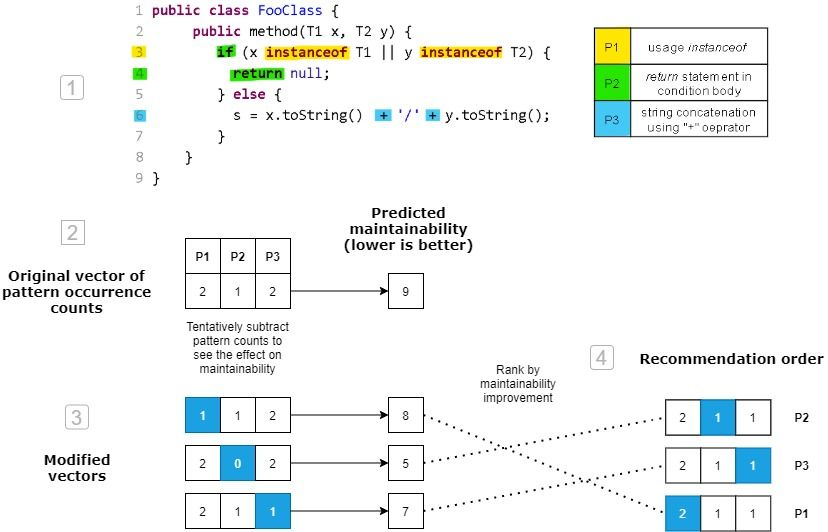
\includegraphics[width=13cm]{how_it_works_diagram_5.jpg}
\centering
\vspace{1 cm}
\caption{How Aibolit works: (1) Inspect the source code for patterns.
(2) Count the pattern occurrences and put them in a vector representation.
Compute the maintainability metric value for the vector.
(3) Consider changes to the vector representation by subtracting pattern counts.
Predict the corresponding maintainbility metric score.
(4) Rank all the alternative vectors wrt to how much they improve the original
maintainability score. Recommend changes that gave the most improvement.}
\label{fig:aibolit_graphic}
\end{figure}

Figure~\ref{fig:aibolit_graphic} represents the Aibolit recommendation proceduce on high level.
In the remaining subsections we provide a more detailed
description of each of Aibolit's components.

\subsection{Patterns \& Quality metrics}
\label{sec:aibolit_patterns_metrics}

\subsubsection*{Patterns}

As discussed above (Section~\ref{sec:related}),
software engineering researchers and practitioners often associate
good and bad code design with specific patterns. We follow this tradition and
build a predictive system to reason about observed patterns in code in terms of their effect on quality.
In the current release of Aibolit, the model is built on top of 34
commonly used manually designed patterns as input features. See Appendix
for the complete list and detailed descriptions. Note that users of Aibolit
can arbitrarily extend the model by implementing and integrating their patterns
of choice.

\subsubsection*{Metrics}

The ultimate goal behind Aibolit's approach is to
learn to identify maintainability-affecting patterns in code and recommend them
to the user. However, as discussed above, maintainability quantification is
still an open problem, and most of the metrics proposed so far typically
describe only a narrow aspect of software maintainability. We recognize it as
the major challenge of our approach and plan to research this problem in the
future.

In the current release of Aibolit, we use Cognitive Complexity \citep{10.1145/3194164.3194186} as
the maintainability metric. We refer to it as the maintainability metric or just
metric in the remainder of the text.

\subsection{Maintainability prediction model}

\label{sec:maint_pred_model}

\subsubsection*{Dataset}

\label{sec:dataset}

To train our prediction model, we mined training data
from Github open source repositories. We chose repositories written in Java
as the main language. We filtered out all non-Java files and all software
testing files. To make sure our data is
representative of good software engineering standards, we only extracted
repositories with at least 100 starts and at least six collaborators.

Aibolit is currently designed to do predictions and recommendations at class
level. For simplicity, we only consider files that contain exactly one
non-abstract Java class.
%We chose this level of granularity because it is intuitive and because we
%wanted to narrow down our scope for the first stage of development. Thus one
%datapoint in our dataset is one Java class.
We filtered out classes with fewer than 50 and more than 300 lines of code.
The resulting filtered dataset consists of 124 repositories and
29,065 classes. Before filtering, we split the dataset into a test and train sets randomy by files with
approximately 0.7:0.3 ratio. The filtered train set contains 20,049 classes,
the filtered test contains 9,016.
%More detailed statistics can be found in Table~\todo. -- keep this for research paper
The complete list of mined repositories and the train/test split is provided in Aibolit
project folder.
%(\todo link to file with repository URLs).

\subsubsection*{Feature and target preprocessing}

Each Java class gets
associated with a vector of numerical features. We use scaled pattern counts as
features. For each pattern from the fixed set
(see Appendix), we count its occurrences in the
class and divide it by the number of non-commented lines in the class (NCSS).
The target value for each datapoint is the maintainability metric value for the
class (Section~\ref{sec:aibolit_patterns_metrics}), also divided by the NCSS.
%(\ref{eq:feat_vector}) and (\ref{eq:targ_val}) summarize feature and target
%value computation (where $f_p^C$ is the feature value for pattern $p$ and code
%$C$, $t^C$ is the target value for code $C$	).
Table~\ref{tab:features_example}
gives an illustration of how a dataset looks like after the this procedure.


%\vspace{0.2in}
%
%\begin{minipage}{.4\linewidth} \begin{equation} \label{eq:feat_vector} f_p^C =
%\frac{\textit{count}(p, C)}{\textit{NCSS}(C)}\end{equation} \end{minipage}%
%\begin{minipage}{.55\linewidth} \begin{equation} \label{eq:targ_val} t^C =
%\frac{\textit{Metric}(C)}{\textit{NCSS}(C)} \end{equation} \end{minipage}
%
%\vspace{0.2in}


We apply NCSS scaling because we observed that our maintainability metric
(Cognitive Complexity) is highly correlated with code size. The scaling
stimulates the model to find more implicit  dependencies between patterns and
complexity.

\begin{table}[H] \begin{center} \begin{tabular}{|r|rrrr|r|} \hline \textbf{class
id} & \textbf{P16} & \textbf{P11} &  \textbf{P13} & \dots & \textbf{CogC}
(target metric) \\ \hline \hline class 1 & 0.008695 & 0.         & 0.026086 &
\dots&  0.417391 \\ class 2 & 0.              & 0.05      & 0.116667 & \dots&
0.466667 \\  class 3 & 0.009909 & 0.         & 0.009909 & \dots & 0.732673 \\
\hline \end{tabular} \end{center} \caption{Example of a training dataset with
preprocessed feature values. \textbf{P16}: {\em Return null}, \textbf{P11}: {\em
Multiple Try},  \textbf{P13}: {\em Null checks}).} \label{tab:features_example}
\end{table}



\subsubsection*{Training}
We train a gradient boosting regression model \citep{Friedman2001GreedyFA}.
We use the implementation of CatBoost \citep{Dorogush2018CatBoostGB} with the RMSE loss function.
For hyperparameter selection, we do a 3-fold crossvalidation.


\subsection{Recommendation algorithm}
\label{sec:recommendation_algorithm}
Our recommendation algorithm ranks
patterns observed in the user's source class according to their individual
impact on the code's maintainability metric value. It then outputs a pattern
with the \textit{most negative impact} as a recommendation to the user to remove
it from their code.

For each pattern $p$ we compute the \textbf{impact factor} $I_{\textit{neg}}(p, C)$
on code $C$, which is intended to capture the \textit{negative
influence} of $p$ on $C$. It is the difference between the quality metric value
of the original code $C$ and the version of $C$ where the count of $p$ has been
decreased (Eq.~\ref{eq:impact_factor}):

\begin{equation} \label{eq:impact_factor} I_{\textit{neg}}(p_i, C) = M(F(C)) -
M(F_{p_{i} - 1}(C)), \end{equation}

where $M$ is a quality metric, $F(C)$ is the feature vector $\langle f^C_{p_1},
..., f^C_{p_n} \rangle$, $F_{p_{i} - 1}(C)$ is the feature vector with the count
of $p_i$ decreased by $1$.%: $\langle f^C_{p_1}, ..., f^C_{p_i - 1}, ...,
%f^C_{p_n} \rangle$. With $f^C_{p_i - 1}$ computed as:\footnote{We chose to
%subtract 1, but in principle it is a hyperparameter of our model and we plan to
%experiment with other values.}

%\begin{equation} \label{eq:feature_count_min_1} f_{p_i - 1}^C =
%\frac{\textit{count}(p_i, C) - 1}{\textit{NCSS}(C)} \end{equation}

Under the ``lower metric is better'' convention (i.e., lower value of quality metric
means better quality), lower values of $I_{\textit{neg}}$ correspond to patterns
that contribute more to the deterioration of the code's quality. We rank pattern
according to their $I_{\textit{neg}}$ and output patterns with lowest values as
recommendations.

Note that at the moment of recommendation we do not observe code with a
decreased pattern count, so we cannot compute the maintainability metric
directly. This is why we resort to a predictive maintainability model
(Section~\ref{sec:maint_pred_model}), which helps estimate maintainability of a
hypothetical code.



\textbf{Algorithm}~\ref{fig:recsys_alg} summarizes how we do recommendations.
For each pattern from the set of patterns used at training, we
precompute feature values and compute the metric value of the source code
(lines~\ref{line:init_F}-\ref{line:compute_m_source}). Then we compute the
impact factor $I_p$ of each pattern $p$ on the source code maintainability
(lines~\ref{line:init_I}-\ref{line:impact}). Under ``lower is better''
convention of maintainability metric, low values of $I_p$ indicate that removal
of $p$ lead to improvement of the metric score. We collect the $K$ most
negatively impacting patterns and output them as recommendations.  Thus, we
 pick patterns $p$ for which $I_p$ are the highest
(lines~\ref{line:topK}-\ref{line:return}).

\begin{algorithm}[t]
\caption{Aibolit recommendation algorithm}
\hspace{\algorithmicindent}
\textbf{Input:}  $\mathsf{M}$: pretrained
maintainability model); $C$: class source code; \\
\hspace{\algorithmicindent} $P$: array of patterns used for training $\mathsf{M}$\\

\begin{algorithmic}[1]
\State $F = [ ]$ \label{line:init_F}
\For{\texttt{i = 1, $|P|$}}
\State $F[i] =\frac{\textit{count}(P[i], C)}{\textit{NCSS}(C)}$% (Eq.~\ref{eq:feat_vector})
\EndFor \State $M_{\textit{observed}} = \mathsf{M}(F)$ \label{line:compute_m_source}
\State $I = [ ]$ \label{line:init_I}
\For{\texttt{i = 1, $|P|$}}

\State $F^{\prime} = F$
\State $F^{\prime}[i] = F[i] - \frac{1}{\textit{NCSS}(C)}$ \label{line:f_prime} %(Eq.~\ref{eq:feature_count_min_1})
\State $I[i] = M_{\textit{observed}} - \mathsf{M}(F^{\prime})$ \label{line:impact} % (Eq.~\ref{eq:impact_factor})
\EndFor
\State $I_{\textit{worst}} = \texttt{topK}_{i \in [1,...,|P|]} (-I[i])$ \label{line:topK}
\State \textbf{return} $\{P[i]~|~i \in I_{\textit{worst}}\}$ \label{line:return}

\end{algorithmic}
\centering
\label{fig:recsys_alg}
\end{algorithm}


% \subsection{How to customize Aibolit} label{sec:customizing_aibolit}

% By design, Aibolit is easily adjustable and extendable. It gives an end user
% the opportunity to adapt the tool to their own requirements and preferences.
% Aibolit's core mechanism is ML-driven, therefore, as the user adds new
% patterns to the system, there is no need to manually specify how the pattern
% should be used by the tool. The interactions between patterns are discovered
% automatically by the learning algorithm.

% In order to modify the set of patterns, the user should provide an
% implementation of a pattern extractor for source code file and modify the
% configuration file (\verb|aibolit/config.py|) accordingly. See full
% instructions in \todo (shouldn't we add them in README?)

% In order to change the quality metric for training the prediction model, ???
% \todo.


\section{Other usage scenarios}
\label{sec:usage_scenarios}
% SPDX-FileCopyrightText: Copyright (c) 2024-2025 Yegor Bugayenko
% SPDX-License-Identifier: MIT

\subsection{Empirical analysis of patterns}

As a by-product of Aibolit's ML and recommendation
engine, we get a tool for empirically analysing different patterns' impacts on the target quality metric. Just
like in the main recommendation algorithm (Algorith~\ref{fig:recsys_alg}, Section~\ref{sec:recommendation_algorithm}), we can estimate whether a particular pattern has a positive or negative impact on the quality metric by considering modifications of source code where pattern count is decreased or increased. We perform such a procedure on a heldout set, which allows to estimate the average impact of a particular pattern on quality.

In Table~\ref{tab:pattern_analysis} we present a case study of the 34 patterns used at training of Aibolit (see Appendix for the pattern descriptions). On a separate test set (see details in Section~\ref{sec:dataset}), for each pattern, we considered increasing and decreasing the pattern's count by 1. We used the pretrained Aibolit's regression model to predict the corresponding change in quality metric.


\begin{table}[ht]
\footnotesize
\begin{tabular}{lllllll}
patterns                                 &   p- m-   &   p+ m+   &   p- m+   &   p+ m-   &   p- m=   &   p+ m=   \\
\\ \hline
Asserts                                	&	92	&	61	&	186	&	219	&	5	&	3	\\
Setters                                		&	245	&	160	&	901	&	976	&	21	&	31	\\
Empty Rethrow                          		&	77	&	65	&	25	&	36	&	0	&	1	\\
Prohibited class name                  		&	617	&	311	&	218	&	522	&	0	&	2	\\
Force Type Casting                     		&	2363	&	2313	&	1742	&	1790	&	14	&	16	\\
Count If Return                        		&	969	&	883	&	214	&	298	&	0	&	2	\\
Implements Multi                       		&	459	&	320	&	264	&	403	&	0	&	0	\\
Instance of                            		&	1396	&	1374	&	151	&	173	&	6	&	6	\\
Many primary constructors              		&	19	&	19	&	604	&	605	&	2	&	1	\\
Method chain                           		&	573	&	574	&	2217	&	2214	&	43	&	45	\\
Multiple try                           		&	371	&	239	&	259	&	391	&	0	&	0	\\
Non final attribute                    		&	1249	&	1185	&	5835	&	5839	&	127	&	187	\\
Null check                             		&	5863	&	5978	&	575	&	457	&	9	&	12	\\
Partial synchronized                   		&	46	&	49	&	155	&	149	&	0	&	3	\\
Redundant catch                        		&	84	&	46	&	38	&	79	&	4	&	1	\\
Return null                            		&	1290	&	813	&	926	&	1401	&	4	&	6	\\
String concat                          		&	1596	&	2089	&	1506	&	1012	&	23	&	24	\\
Super Method                           		&	212	&	275	&	1012	&	949	&	10	&	10	\\
This in constructor                    		&	15	&	42	&	72	&	45	&	0	&	0	\\
Var declaration distance for 5 lines   		&	1976	&	1464	&	738	&	1244	&	19	&	25	\\
Var declaration distance for 7 lines   		&	1190	&	959	&	733	&	949	&	16	&	31	\\
Var declaration distance for 11 lines  		&	703	&	603	&	365	&	466	&	10	&	9	\\
Var in the middle                      		&	3372	&	3117	&	2799	&	3046	&	37	&	45	\\
Array as function argument             		&	882	&	768	&	351	&	464	&	1	&	2	\\
Joined validation                      		&	232	&	226	&	14	&	26	&	8	&	2	\\
Non final class                        		&	7141	&	3201	&	3723	&	7663	&	0	&	0	\\
Private static method                  		&	529	&	541	&	667	&	648	&	2	&	9	\\
Public static method                   		&	1166	&	1212	&	1142	&	1088	&	4	&	12	\\
Null Assignment                        		&	1245	&	803	&	717	&	1150	&	6	&	15	\\
Multiple While                         		&	120	&	97	&	16	&	39	&	0	&	0	\\
Protected Method                       		&	868	&	402	&	1147	&	1613	&	7	&	7	\\
Send Null                              		&	556	&	325	&	1510	&	1733	&	5	&	13	\\
Nested Loop                            		&	580	&	527	&	29	&	81	&	1	&	2	\\
\hline
\end{tabular}
\centering
\caption{Empirical analysis of patterns. For each source code in the test set, we consider encreasing (\textbf{p+}) and decreasing (\textbf{p-}) pattern count by 1. And we recorded whether the maintainability metric increased (\textbf{m+}) or decreased (\textbf{m-}) as a result of that (where lower is better). In some cases the metric did no change (\textbf{m=}). The values in the cells are counts of cases.}
\label{tab:pattern_analysis}
\captionsetup{font=scriptsize}
% \caption*{
%     We use the following notation into named columns:
%     ($p-$): decrease pattern by $\frac{1}{ncss}$;
%     ($p+$): increase pattern by $\frac{1}{ncss}$;
%     ($c-$): complexity has been decreased; $c+$: complexity has been increased;
%     ($c=$): complexity has been not changed;
%     (\emph{-1(top1)}): decreasing of pattern shows best \emph{CogC} improvement;
%     (\emph{+1(top1)}): increasing of pattern shows best \emph{CogC} improvement.
% }
% \caption*{
%     We use the following notation into named columns: \\
%     \\
%     \centering
%     \begin{tabular}{rl}
%         $p-$ & decrease pattern by $\frac{1}{ncss}$ \\
%         $p+$ & increase pattern by $\frac{1}{ncss}$ \\
%         $c-$ & complexity has been decreased \\
%         $c+$ & complexity has been increased \\
%         $c=$ & complexity has been not changed \\
%         \emph{-1(top1)} & decreasing of pattern shows best \emph{CogC} improvement   \\
%         \emph{+1(top1)} & increasing of pattern shows best \emph{CogC} improvement \\
%     \end{tabular}
% }
\end{table}

Based on the statistics in Table~\ref{tab:pattern_analysis}, it appears that \emph{Prohibited class name}, \emph{Count If Return}, \emph{Instance of}, \emph{Null check}, \emph{Nested Loop},
\emph{Array as function argument}, \emph{Joined validation} are \textbf{anti-patterns}, since their count decrease tends to improve  the metric. Another group of patterns are \emph{Setters}, \emph{Many primary constructors}, \emph{Method chain}, \emph{Non final attribute}, \emph{Super Method}, \emph{Send Null patterns}: for them we observe that decresing them causes the metric to deteriorate, and increasing causes the metric to improve. We consider them \textbf{pro-patterns}. The third group (the rest of the patterns) can both improve and deteriorate the metric. We restrain oursevles from calling them either anti- or pro-patterns.

Attempting to interpret the results, we observe that ``true'' anti-patterns usually have \emph{if/else condition} or cycle in their definition.
E.g., \emph{Null check} always checks for a null, \emph{Count If Return}, \emph{Instance of},
\emph{Joined validation} have always \emph{if condition}, \emph{Nested Loop} has always at least 1 loop inside. Given that so far we have worked with the Cognitive Complexity metric, it is no surprise that those patterns affect it (\emph{if/else condition} or cycle are the main contributors into \emph{CogC}). Despite this limitation of the present analysis, we believe the proposed \textit{method} itself can be very useful in software engineering practice and research.




% ORIG TABLE:
% patterns                                & -1(top1)  & +1(top1)  &   p- m-   &   p+ m+   &   p- m+   &   p+ m-   &   p- m=   &   p+ m=   \\
% \\ \hline
% Asserts                                 &   0   &   100 &   92  &   61  &   186 &   219 &   5   &   3   \\
% Setters                                 &   1   &   113 &   245 &   160 &   901 &   976 &   21  &   31  \\
% Empty Rethrow                           &   1   &   4   &   77  &   65  &   25  &   36  &   0   &   1   \\
% Prohibited class name                   &   80  &   24  &   617 &   311 &   218 &   522 &   0   &   2   \\
% Force Type Casting                      &   69  &   24  &   2363    &   2313    &   1742    &   1790    &   14  &   16  \\
% Count If Return                         &   311 &   26  &   969 &   883 &   214 &   298 &   0   &   2   \\
% Implements Multi                        &   24  &   244 &   459 &   320 &   264 &   403 &   0   &   0   \\
% Instance of                             &   211 &   6   &   1396    &   1374    &   151 &   173 &   6   &   6   \\
% Many primary constructors               &   0   &   343 &   19  &   19  &   604 &   605 &   2   &   1   \\
% Method chain                            &   3   &   203 &   573 &   574 &   2217    &   2214    &   43  &   45  \\
% Multiple try                            &   156 &   180 &   371 &   239 &   259 &   391 &   0   &   0   \\
% Non final attribute                     &   34  &   485 &   1249    &   1185    &   5835    &   5839    &   127 &   187 \\
% Null check                              &   1573    &   14  &   5863    &   5978    &   575 &   457 &   9   &   12  \\
% Partial synchronized                    &   1   &   93  &   46  &   49  &   155 &   149 &   0   &   3   \\
% Redundant catch                         &   6   &   2   &   84  &   46  &   38  &   79  &   4   &   1   \\
% Return null                             &   104 &   40  &   1290    &   813 &   926 &   1401    &   4   &   6   \\
% String concat                           &   43  &   126 &   1596    &   2089    &   1506    &   1012    &   23  &   24  \\
% Super Method                            &   1   &   174 &   212 &   275 &   1012    &   949 &   10  &   10  \\
% This in constructor                     &   2   &   891 &   15  &   42  &   72  &   45  &   0   &   0   \\
% Var declaration distance for 5 lines    &   396 &   14  &   1976    &   1464    &   738 &   1244    &   19  &   25  \\
% Var declaration distance for 7 lines    &   25  &   95  &   1190    &   959 &   733 &   949 &   16  &   31  \\
% Var declaration distance for 11 lines   &   16  &   686 &   703 &   603 &   365 &   466 &   10  &   9   \\
% Var in the middle                       &   118 &   50  &   3372    &   3117    &   2799    &   3046    &   37  &   45  \\
% Array as function argument              &   86  &   25  &   882 &   768 &   351 &   464 &   1   &   2   \\
% Joined validation                       &   63  &   2   &   232 &   226 &   14  &   26  &   8   &   2   \\
% Non final class                         &   1056    &   2370    &   7141    &   3201    &   3723    &   7663    &   0   &   0   \\
% Private static method                   &   35  &   133 &   529 &   541 &   667 &   648 &   2   &   9   \\
% Public static method                    &   37  &   408 &   1166    &   1212    &   1142    &   1088    &   4   &   12  \\
% Null Assignment                         &   103 &   35  &   1245    &   803 &   717 &   1150    &   6   &   15  \\
% Multiple While                          &   65  &   7   &   120 &   97  &   16  &   39  &   0   &   0   \\
% Protected Method                        &   71  &   151 &   868 &   402 &   1147    &   1613    &   7   &   7   \\
% Send Null                               &   13  &   109 &   556 &   325 &   1510    &   1733    &   5   &   13  \\
% Nested Loop                             &   412 &   35  &   580 &   527 &   29  &   81  &   1   &   2   \\

\subsection{Aibolit Index}

In addition to the recommendation functionality, we designed a feature to measure the overall quality of developer's source code, \textit{Aibolit Index}.
It is is a single number, with following properties: 
\begin{itemize}
\item[(i)] the more patterns are suggested to fix, the higher Aibolit Index;
\item[(ii)] the higher negative impact factor (see Section \ref{sec:recommendation_algorithm}) 
of detected patterns the higher Aibolit Index.
\end{itemize}
Therefore, the lower Abolit Index the better the project's code from the point 
of view of Aibolit.

Let $P(C)$ be a set of all patterns Aibolit recommends to fix for Java class $C$.
% As we know from the section ~\ref{sec:recommendation_algorithm}, each 
% recommended anti-pattern $p \in P(C)$ has an associated impact factor $I_{p}$ and a count $count(p, C)$.
We define the Aibolit Index $A(C)$ of Java class $C$ as a sum of the products of
impact factors $I_{p}$ and scaled counts $count(p, C)$ for all of the 
patterns occurring in the class (Eq.~\ref{eq:aibolit_index}). We use log-scaling for smoothing purposes, because some patterns are a lot more common than others.    


\begin{equation}
    A(C) = \sum_{p \in P(C)} { I_{p}(C) \cdot \ln{(count(p, C) + 1)} } \label{eq:aibolit_index}
\end{equation}


The Aibolit Index of a project is defined as average Aibolit Index
across all Java classes in the project. In Table~\ref{table:aibolit_index_repos} 
you can see a calculated Aibolit Index of some GitHub Java repositories with 
more than 4500 stars. Aibolit Index is supposed to be a convenient instrument
to get a first estimate of the project code's quality. 

\begin{table}[t]
\footnotesize
    \begin{tabular}{|l|l|l|l|l|l|l|}
    \hline
    Repository & Aibolit Index & Total files & Total NCSS & GitHub stars \\ 
    \hline
    ReactiveX\textbackslash RxJava& 6.66& 1493& 25270 & 42972  \\
    bumptech\textbackslash glide& 5.81& 465& 5078 & 29364 \\
    JakeWharton\textbackslash butterknife& 6.31& 74& 935 & 25347  \\
    greenrobot\textbackslash EventBus& 7.48& 51& 651 & 22637  \\
    skylot\textbackslash jadx& 6.69& 602& 12658 & 22602 \\
    alibaba\textbackslash fastjson & 9.97& 144& 20175 & 21891 \\
    alibaba\textbackslash druid & 6.36& 822& 28852 & 21581 \\ 
    Netflix\textbackslash Hystrix& 6.74& 292& 2920 & 19888 \\
    ReactiveX\textbackslash RxAndroid& 5.47& 9& 59 & 19010 \\
    google\textbackslash gson& 6.87& 160& 2941 & 18084 \\
    square\textbackslash picasso& 6.21& 26& 687 & 17514 \\
    libgdx\textbackslash libgdx & 5.02 & 1981 & 46409 & 17105 \\
    nostra13\textbackslash Android-Universal-Image-Loader& 7.84& 62& 1059 & 16722  \\
    qiurunze123\textbackslash miaosha& 3.57& 197& 841 & 16224 \\
    wuyouzhuguli\textbackslash SpringAll& 13.41& 467& 463 & 15221 \\
    justauth\textbackslash JustAuth& 4.36& 46& 241 & 8916 \\
    heibaiying\textbackslash BigData-Notes& 11.17& 54& 204 & 7166  \\
    crossoverJie\textbackslash cim & 6.70& 96& 574 & 5841 \\
    wildfirechat\textbackslash server& 6.51& 285& 4671  & 5140 \\
    febsteam\textbackslash FEBS-Shiro & 5.66& 90& 453 & 4777 \\
    \hline
    \end{tabular}
    \centering
\caption{Aibolit Index of some popular Java repositories. \label{table:aibolit_index_repos}}
\end{table}








\section{Conclusion \& Future Work}
\label{sec:conclusion}
% SPDX-FileCopyrightText: Copyright (c) 2019-2025 Aibolit
% SPDX-License-Identifier: MIT

Aibolit is a recommender system that helps improve the quality of Java classes.
The recommendations are learned from OSS Java projects using ML methods.
Aibolit provides ranked recommendations for each specific Java class,
which differs Aibolit from others style checkers and makes it unique.

Aibolit is an extendable system, allowing anyone to add new patterns and to
increase the training dataset and thus improve the precision and usefulness
of recommendations. Aibolit can also be used as a framework for analysis of
patterns and to decide whether any pattern, however subjective it is, is an anti- or a pro-pattern
with respect to a particular quality metric. As a complementary result,
we contribute a 100K+ dataset of patterns and metrics calculated for Java classes.

The first version of Aibolit is relatively simple and there is room
for improvement. If the anti-pattern has found, we recommend to fix all instances
of the pattern in the code. Instead, we may consider each specific occurrence of the pattern.
We may exploit its relative position in the structure of the code, rather than just count
the frequency. Moreover, Aibolit inspects each Java class independently. But
we might consider the relations between classes in the future. Furthermore,
Aibolit's prediction model relies on patterns only. In order to improve the model,
we have to think about additional features, for example, information about
project domain or used frameworks.

Aibolit is a firm step toward the next generation of tools to control
and improve software quality. It is a complementary tool for
product owners who already use tools to manage software quality.


\newpage
\AtNextBibliography{\small}
\setstretch{1.0}
\raggedright
\begin{multicols}{2}\printbibliography\end{multicols}

\newpage
\section*{Appendix}
\label{sec:appendix}
% SPDX-FileCopyrightText: Copyright (c) 2024-2025 Yegor Bugayenko
% SPDX-License-Identifier: MIT

\subsection*{Patterns Dictionary}

\begin{itemize}
	\item \pattern{Assert in code}{P1}
	{If there is an assert statement in code block, and name of class doesn't end with Test, it is considered a pattern.}
	{\it Example:}
\begin{lstlisting}[language=Java]
class Book {
	void foo(String x) {
	assert x != null; // here
}
\end{lstlisting}

	\item \pattern{Setter}{P2}{The method's name starts with set, then goes the name of the attribute. There are attributes assigning in the method. Also, asserts are ignored.}
	{\it Examples:}
\begin{lstlisting}[language=Java]
class Book {
	private String title;
	void setTitle(String) {
		this.title = t;
	}
}
\end{lstlisting}

\begin{lstlisting}[language=Java]
class Book {
	private String title;
	public void setIsDiscrete() {
		assert !isDiscrete;
		assert !x; //ignore it
		this.isDiscrete = isDiscrete;
	}
}
\end{lstlisting}

\begin{lstlisting}[language=Java]
class Book {
private String isDiscrete;

	public void setIsDiscrete(String isDiscretem, boolean x) {
		assert !isDiscrete;
		assert !x; //ignore it
		this.isDiscrete = isDiscrete;
	}
}
\end{lstlisting}

\begin{lstlisting}[language=Java]
class Book {
	private String title;

	@Override
	synchronized public void setConf(Configuration conf) {
		this.conf = conf;
		this.randomDevPath = conf.get(
		HADOOP_SECURITY_SECURE_RANDOM_DEVICE_FILE_PATH_KEY,
		HADOOP_SECURITY_SECURE_RANDOM_DEVICE_FILE_PATH_DEFAULT);
		close(); \\ some minor changes also do not affect, it is still Setter pattern
	}
}
\end{lstlisting}

	\item \pattern{Empty Rethrow}{P3}{We throw the same exception as it was caught.}
	{\it Example:}
\begin{lstlisting}[language=Java]
class Book {
	void foo() {
		try {
			File.readAllBytes();
		} catch (IOException e) {
			// maybe something else here
			throw e; // here!
		}
	}
}
\end{lstlisting}

	\item \pattern{ErClass}{P4}{ If a class name is one of the following (or ends with this word), it's the pattern:

		Manager, Controller, Router, Dispatcher, Printer, Writer, Reader, Parser, Generator, Renderer, Listener, Producer, Holder, Interceptor.}

	\item \pattern{Force type casting}{P5}{The force type casting considered as a pattern.}
	{\it Example:}
\begin{lstlisting}[language=Java]
// casting to int is
public int square (int n) {
	return (int) java.lang.Math.pow(n,2);
}
\end{lstlisting}

	\item \pattern{If return if detection}{P6}{If there is a return in if condition, it's a pattern.}
	{\it Example:}
	\begin{lstlisting}[language=Java]
class T1 {
	public void main(int x) {
		if (x < 0) {
			return;
		} else {
			System.out.println("X is positive or zero");
		}
	}
}
\end{lstlisting}

	\item \pattern{Implements Multi}{P7}{If a class implements more than 1 interface it's a pattern.}
	{\it Examples:}
	\begin{lstlisting}[language=Java]
public class AnimatableSplitDimensionPathValue implements AnimatableValue<PointF, PointF> {
	private final AnimatableFloatValue animatableXDimension;
	private final AnimatableFloatValue animatableYDimension;

	public AnimatableSplitDimensionPathValue(
	AnimatableFloatValue animatableXDimension,
	AnimatableFloatValue animatableYDimension) {
		this.animatableXDimension = animatableXDimension;
		this.animatableYDimension = animatableYDimension;
	}
}
\end{lstlisting}
\begin{lstlisting}[language=Java]
public class a implements A, B {
}
\end{lstlisting}

	\item \pattern{Using \texttt{instanceof} operator}{P8}{ Using of \texttt{instanceof} operator considered as pattern.}
{\it Examples:}
	\begin{lstlisting}[language=Java]
public static void main(String[] args) {
	Child obj = new Child();
	if (obj instanceof String)
		System.out.println("obj is instance of Child");
}
\end{lstlisting}
\begin{lstlisting}[language=Java]
class Test
{
	public static void main(String[] args)
	{
		Child cobj = new Child();
		System.out.println(b.getClass().isInstance(c));
	}
}
\end{lstlisting}

	\item \pattern{Many primary ctors}{P9}{If there is more than one primary constructors in a class, it is considered a pattern.}
	{\it Example:}
\begin{lstlisting}[language=Java]
class Book {

	private final int a;
	Book(int x) { // first primary ctor
		this.a = x;
	}
	Book() { // second
		this.a = 0;
	}
}
\end{lstlisting}

	\item \pattern{Usage of method chaining more than one time}{P10}{If we use more than one method chaining invocation.}
{\it Example:}
\begin{lstlisting}[language=Java]
// here we use method chaining 4 times
public void start() {
	MyObject.Start()
	.SpecifySomeParameter()
	.SpecifySomeOtherParameter()
	.Execute();
}
\end{lstlisting}

	\item \pattern{Multiple Try}{P11}{Once we see more than one try in a single method, it's a pattern.}
{\it Example:}
\begin{lstlisting}[language=Java]
class Foo {
	void bar() {
		try {
			// some code
		} catch (IOException ex) {
			// do something
		}
			// some other code
		try {  // here!
			// some code
		} catch (IOException ex) {
			// do something
		}
	}
}
\end{lstlisting}

	\item \pattern{Non final attributes}{P12}{Once we see a mutable attribute (without final modifier), it's considered a pattern.}
{\it Example:}
\begin{lstlisting}[language=Java]
class Book {
	private int id;
	// something else
}
\end{lstlisting}

	\item \pattern{Null checks}{P13}{If we check that something equals (or not equals) null (except in constructor) it is considered a pattern.}
{\it Example:}
\begin{lstlisting}[language=Java]
class Foo {
	private String z;
	void x() {
		if (this.z == null) { // here!
			throw new RuntimeException("oops");
		}
	}
}
\end{lstlisting}

	\item \pattern{Partial synchronized}{P14}{Here, the synchronized block doesn't include all statements of the method. Something stays out of the block.}
{\it Example:}
\begin{lstlisting}[language=Java]
class Book {
	private int a;
	void foo() {
		synchronized (this.a) {
			this.a = 2;
		}
		this.a = 1; // here!
	}
}
\end{lstlisting}

	\item \pattern{Redundant catch}{P15}{Here, the method \texttt{foo()} throws IOException, but we catch it inside the method.}
{\it Example:}
\begin{lstlisting}[language=Java]
class Book {
	void foo() throws IOException {
		try {
			Files.readAllBytes();
		} catch (IOException e) { // here
			// do something
		}
	}
}
\end{lstlisting}

	\item \pattern{Return null}{P16}{When we return null, it's a pattern.}
{\it Example:}
\begin{lstlisting}[language=Java]
class Book {
	String foo() {
		return null;
	}
}
\end{lstlisting}

	\item \pattern{String concatenation using \texttt{+} operator}{P17}{Any usage string concatenation using \texttt{+} operator is considered as pattern match.}
{\it Example:}
\begin{lstlisting}[language=Java]
public void start() {
	// this line is match the pattern
	System.out.println("test" + str1 + "34234" + str2);
	list = new ArrayList<>();
	for (int i = 0; i < 10; i++)
		list.add(Boolean.FALSE);
}
\end{lstlisting}

	\item \pattern{Override method calls parent method}{P18}{If we call parent method from override class method it is considered as the pattern.}
{\it Example:}
\begin{lstlisting}[language=Java]
@Override
public void method1() {
	System.out.println("subclass method1");
	super.method1();
}
\end{lstlisting}

	\item \pattern{Class constructor except \texttt{this} contains other code}{P19}{The first constructor has this() and some other statements. This is the ``hybrid constructor'' pattern.}
{\it Example:}
\begin{lstlisting}[language=Java]
class Book {
	private int id;
	Book() {
		this(1);
		int a = 1; // here
	}
	Book(int i) {
		this.id = I;
	}
}
\end{lstlisting}

	\item \pattern{Line distance between variable declaration and first usage greater then threshold}{P20\_5, P20\_7, P20\_11}{If line distance between variable declaration and first usage exceeds some threshold we consider it as the pattern. We calculate only non-empty lines. P20\_5 means that distance is 5.}
{\it Example:}
\begin{lstlisting}[language=Java]
// variable a declared and used with 2 lines distance
static void myMethod() {
	string path1 = '/tmp/test1';
	int a = 4;

	string path2 = '/tmp/test2';
	string path3 = '/tmp/test3';
	a = a + 4;
}
\end{lstlisting}

	\item \pattern{Variable is declared in the middle of the method body}{P21}{All variable we need have to be declared at the beginning of its scope. If variable declared inside the scope following after logical blocks we consider that this is the pattern.}
{\it Example:}
\begin{lstlisting}[language=Java]
// The declaration of variable list is match pattern.
static void myMethod2() {
	int b = 4;
	b = b + 6;
	List<Integer> list = new List<Integer>();
}
\end{lstlisting}

	\item \pattern{Array as argument}{P22}{If we pass an array as an argument, it's a pattern. It's better to use objects, instead of arrays.}
{\it Example:}
\begin{lstlisting}[language=Java]
class Foo {
	void bar(int[] x) {
	}
}
\end{lstlisting}

	\item \pattern{Joined Validation}{P23}{Once you see a validation (if with a single throw inside) and its condition contains more than one condition joined with OR -- it's a pattern.}
{\it Example:}
\begin{lstlisting}[language=Java]
class Book {
	void print(int x, int y) {
		if (x == 1 || y == 1) { // here!
			throw new Exception("Oops");
		}
	}
}
\end{lstlisting}

	\item \pattern{Class declaration must always be \texttt{final}}{P24}{Once you see a non \texttt{final} method, it's a pattern.}
{\it Example:}
\begin{lstlisting}[language=Java]
class Book {
	private static void foo() {
	}
}
\end{lstlisting}

	\item \pattern{Private static method}{P25}{Once you see a \texttt{private static} method, it's a pattern.}
{\it Example:}
\begin{lstlisting}[language=Java]
class Book {
	private static void foo() {
		//something
	}
}
\end{lstlisting}

	\item \pattern{Public static method}{P26}{Once you see a \texttt{public static} method, it's a pattern.}
{\it Example:}
\begin{lstlisting}[language=Java]
class Book {
	private static void foo() {
		//something
	}
}
\end{lstlisting}

	\item \pattern{Var siblings}{P27}{Here fileSize and fileDate are ``siblings'' because they both have file as first part of their compound names. It's better to rename them to size and date.\\
		file and fileSize are NOT siblings.}
{\it Example:}
\begin{lstlisting}[language=Java]
class Foo {
	void bar() {
		int fileSize = 10;
		Date fileDate = new Date();
	}
}
\end{lstlisting}

	\item \pattern{Assign null}{P28}{Once we see \texttt{= null}, it's a pattern.}
{\it Example:}
\begin{lstlisting}[language=Java]
class Foo {
	void bar() {
		String a = null; // here
	}
}
\end{lstlisting}

	\item \pattern{Multiple \texttt{while} pattern}{P29}{Once you see two or more \texttt{while} statements in a method body, it's a pattern.}
{\it Example:}
\begin{lstlisting}[language=Java]
class Book {
	void foo() {
		while (true) {
		}
		// something
		while (true) {
		}
	}
}
\end{lstlisting}

	\item \pattern{Protected method}{P30}{Once we find a protected method in a class, it's a pattern.}

	\item \pattern{Send \texttt{null}}{P31}{Once we see that \texttt{null} is being given as an argument to some method, it's a pattern.}
{\it Example:}
\begin{lstlisting}[language=Java]
class Foo {
	void bar() {
		FileUtils.doIt(null); // here
	}
}
\end{lstlisting}

	\item \pattern{Nested loop}{P32}{Once we find a loop (\texttt{for} / \texttt{while}) inside another loop it's a pattern.}
{\it Example:}
\begin{lstlisting}[language=Java]
class Foo {
	void foo() {
		white (true) {
			for (;;) { // here
			}
		}
	}
}
\end{lstlisting}

\end{itemize}


\end{document}
